% based on the ACM article example, extracted from here: https://www.acm.org/sigs/publications/proceedings-templates
\documentclass{acm_proc_article-sp}

\usepackage[utf8]{inputenc}
\usepackage[T1]{fontenc}
\usepackage{url}
\usepackage{multicol}
\usepackage{mathtools}
\usepackage{amssymb}
\usepackage{amsmath}
\usepackage{amsfonts}
\usepackage{graphics}
\usepackage{listings}
\usepackage{listingsutf8}
\usepackage{setspace}
\usepackage{xcolor}
\lstset{inputencoding=utf8/latin1}

\begin{document}

\title{VOIP}
\subtitle{El encuentro de un sistema anticuado con su mayor némesis}
\numberofauthors{1}

\author{
  \alignauthor
  García Ruth\\
  \affaddr{Universidad Mayor de San Andrés}\\
  \affaddr{Carrera de Informática}\\
  \email{vengadoravg@gmail.com}
}
\date{\today}

\maketitle
\begin{abstract}
Este artículo pretende ser una poco-ambiciosa recopilación de información sobre las regulaciones contra la VoIP de algunas compañías y gobiernos.

Comenzando con un trasfondo histórico, rememorando los '70s durante el nacimiento de la caja azul, continuando con una corta explicación sobre el funcionamiento de la VoIP, y finalizando con una pequeña recopilación de restricciones y regulaciones por compañías y gobiernos, en su afán por permanecer controlando y/o monetizando las comunicaciones de las personas.

\end{abstract}

\keywords{VoIP, surveillance, restricción, regulación, llamadas gratis}

\section{Introduction}
Entre 1960 y 1970, un grupo de \textit{hackers}\footnote{El término ``hácker'' ha sido tergiversado a través de los tiempos. En este artículo, se usará el término ``hácker'', refiriéndose al espíritu original, tal como nació en el MIT, durante 1961. Es decir, refiriéndose a aquellas personas que disfrutan de jugar con la tecnología, amoldándola y, en ocasiones, rompiéndola para que funcione de una forma en la que no fue planeada.}, leyendo publicaciones sobre el funcionamiento de las frecuencias usadas para realizar llamadas hechas por Bell, descubrieron cómo funcionaban los teléfonos. \cite{bluebox:sarts}

Con insasiable sed de conocimiento, y con bastos conocimientos en electrónica adquiridos durante muchas jornadas de \textit{hacking}, crean un aparato que permite realizar llamadas de forma gratuita: \textit{La Caja Azul}.

\begin{figure}
\centering
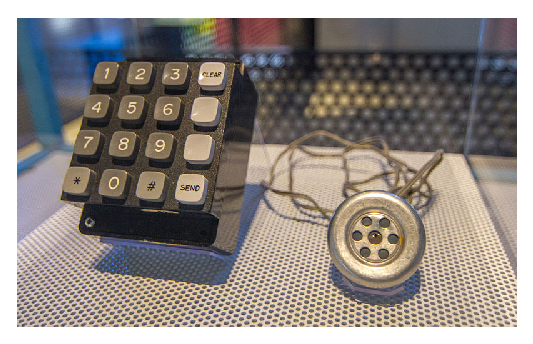
\epsfig{file=assets/bluebox.eps}
\caption{Un \textit{Blue Box} en el museo de \textit{Powerhouse}.
Autor: Maksym Kozienko}
\end{figure}

Varios meses después, Bell se da cuenta de las consecuencias que toda esta información publicada podrían causar, y destruyó físicamente las páginas en las que se encontraba toda esta información, sin embargo ya era muy tarde, porque los háckers ya habían digerido el conocimiento.

Indudablemente, los dueños de las empresas de telecomunicaciones estaban enojados y buscaban culpables, y descargaron toda su ira en los pocos háckers que pudieron atrapar e incriminar. Entre ellos estaba Kevin Mitnick, cuya historia es muy conocida. Kevin Mitnick fue acusado de ser capaz de desencadenar una guerra nuclear si se le permitía acceso a un teléfono.

La ira de estos empresarios estaba parcialmente justificada. Darle mantenimiento a todo este sistema telefónico era caro e ineficaz por entonces. El internet a la velocidad que hoy se consideraría ``normal'', por entonces era un lujo al que solo personas con el conocimiento suficiente, y con el dinero suficiente podían acceder.\cite{bluebox:documentary}

Hoy en día, con el internet a la vuelta de la esquina, el beneficio de las ``llamadas gratuitas'' ya no perjudica a nadie, dando a luz al VoIP: \textit{Voice over Internet Protocol}.

Pese a esto, muchas compañías de telefonía aún ven a las ``llamadas gratuitas'' como una abominable blasfemia a su seguridad financiera, y cuál si fuera el fruto prohibido del Edén, intentan restringir y regular su uso.


\section{Funcionamiento}
\subsection{Definición}
VoIP es un acrónimo que viene de: \textit{\textbf{V}oice \textbf{o}ver \textbf{I}nternet \textbf{P}rotocol}, que significa: ``voz sobre IP''. Es un término que se usa para identificar a todos aquellos métodos que sirven para proveer servicios telefónicos a través de la Internet.\cite{voip:whatis}

Es importante notar que VoIP no es un protocolo, ni un método; VoIP no define la forma en la que una persona usa servicios telefónicos a través de la Internet, es solo un término usado para identificar a ese conjunto de métodos que hacen este servicio posible.\cite{voip:rfc}

Sin embargo, se pueden identificar 3 métodos principales para realizar VoIP:

\begin{itemize}
\item \textbf{ATA:} (Analogue Terminal Adapter) Es una especie de router que usa para conectar teléfonos analógicos (como los usados para realizar llamadas por linea fija en los planes de COTEL).\cite{voip:ata}
\item \textbf{IP Phone:} Es un teléfono especial, que a simple vista, parece un teléfono normal, pero tiene un puerto Ethernet, mediante el cuál se conecta a un servidor VoIP, que hace posible una llamada por Internet.
\item \textbf{\textit{softphone:}} Las llamadas se realizan mediante software. Se pretende que un dispositivo inteligente (como una computadora, o un smartphone) imite la función de un PSTN (\textit{Public Switched Telephone Network}, que es el término usado para identificar un teléfono tradicional).
\end{itemize}

Todos estos métodos pueden ser integrados con PSTN, sin embargo, esta integración no es requisito indispensable de VoIP. Telegram, Lime y Whatsapp es un softphone que permite VoIP, por ejemplo. 

\subsection{Protocolos}

Todo método para realizar VoIP, requiere de un protocolo. Una de las funciones de este protocolo es traducir las señales analógicas telefónicas en señales digitales que puedan ser transferidas mediante el internet.

Existe una gran variedad de protocolos, muchos de ellos permiten la comunicación encriptada. Entre ellos, está SIP: Session Initiation Protocol, que es un protocolo para llevar a cabo \textit{sesiones} con uno o más participantes. Estas incluyen llamadas telefónicas por internet, distribución multimedia y conferencias multimedia.\cite{rfc:sip}



\section{Restricciones y Regulaciones}
\begin{figure}
\centering
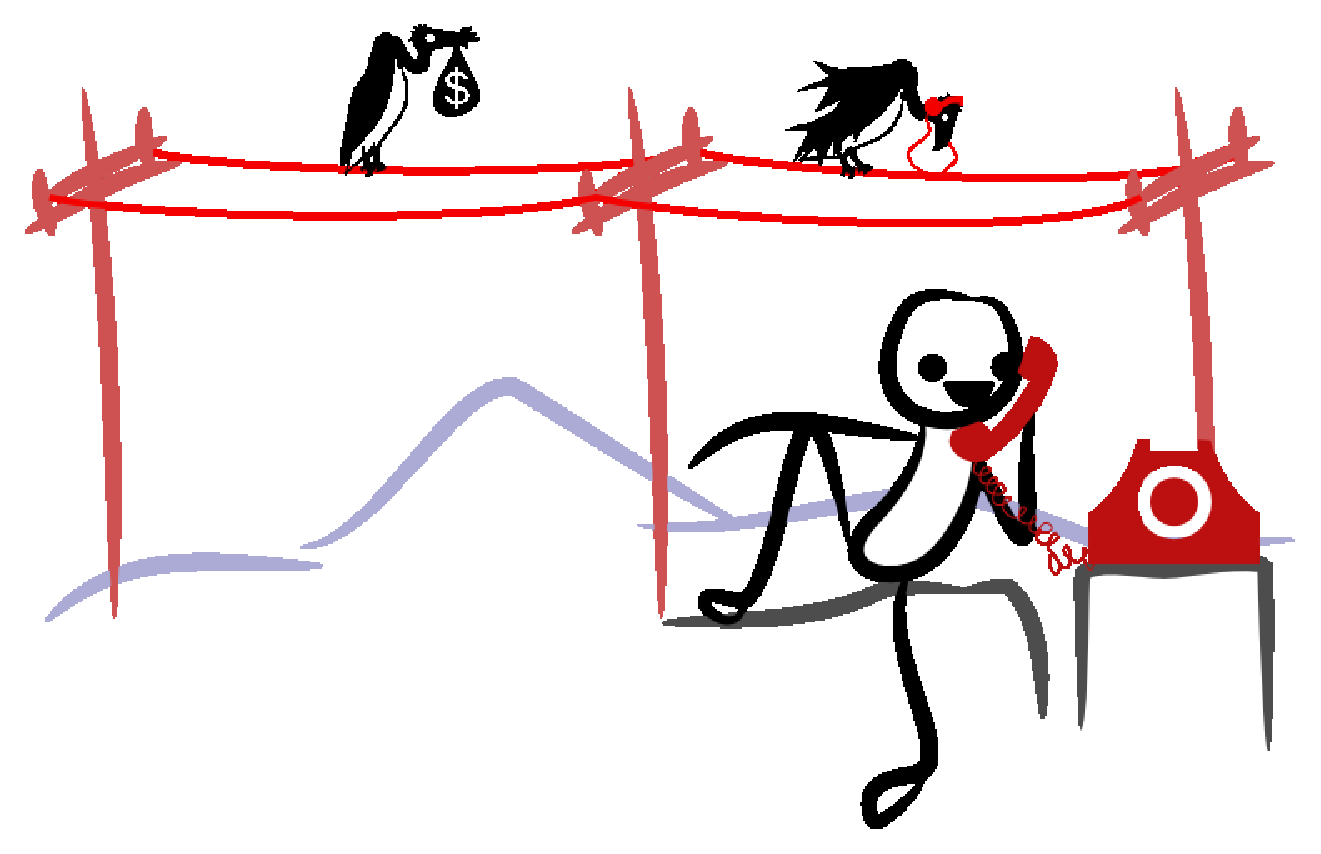
\epsfig{file=assets/buitres.eps, width=0.4\textwidth}
\caption{El gobierno y las empresas se benefician de nuestras telecomunicaciones: tanto monetariamente, como mediante el \textit{surveillance}. El VoIP tiene un costo bajo y provee una comunicación segura, ya que puede ser encriptada. Arte del buitre por Ocal\cite{clker:ocal}}
\end{figure}

\quote{1. La cultura siempre se construye en el pasado.\\
2. El pasado siempre intenta controlar el futuro.\\
3. Nuestro futuro se está volviendo menos libre.\\
4. Para construir sociedades libres, debes limitar el control del pasado.}
\cite{rip:manifesto}

En India al 2014, airtel, la compañía más grande de telecomunicaciones de ese lugar, comenzó a cobrar extra por el servicio de VoIP desde celulares, utilizando servicios como Skype, Viber, Google Hangouts, entre otros, pese a que usar los servicios VoIP es mucho menos costoso que realizar llamadas usando PSTN.\cite{airtel}

En Oman está penado con una multa de 130,317 dólares estadounidenses, y dos años en prisión, realizar llamadas mediante VoIP. En 2009, 212 personas fueron penalizadas por usar VoIP en un café internet.\cite{oman}

En Corea del Sur sólamente se permite usar servicios VoIP autorizados. El costo es muy parecido al de las llamadas mediante PSTN.\cite{korea}

En Estados Unidos, es permitido que las autoridades escuchen conversaciones sobre VoIP sin una orden.\cite{usa}


%
% The following two commands are all you need in the
% initial runs of your .tex file to
% produce the bibliography for the citations in your paper.
\bibliographystyle{abbrv}
\bibliography{RMG-207665722}  % sigproc.bib is the name of the Bibliography in this case
% You must have a proper ".bib" file
%  and remember to run:
% latex bibtex latex latex
% to resolve all references
%
% ACM needs 'a single self-contained file'!
%
%APPENDICES are optional

\balancecolumns
% That's all folks!
\end{document}
